\chapter{Progettazione e Realizzazione di un Ambiente per la Configurazione Avanzata}\label{capitolo:progettazione_realizzazione}
\markboth{Progettazione e Realizzazione}{}
Questo capitolo è dedicato alla comprensione e descrizione delle fasi di progettazione e realizzazione di \visualnetkit{}. Verrà mostrata in maniera dettagliata la nuova struttura dei \plugin{} accennata nel precedente capitolo, e successivamente, verranno descritte le altre porzioni del sistema, analizzando i singoli moduli che lo compongono.

\begin{figure}[!htb]
	\centering
	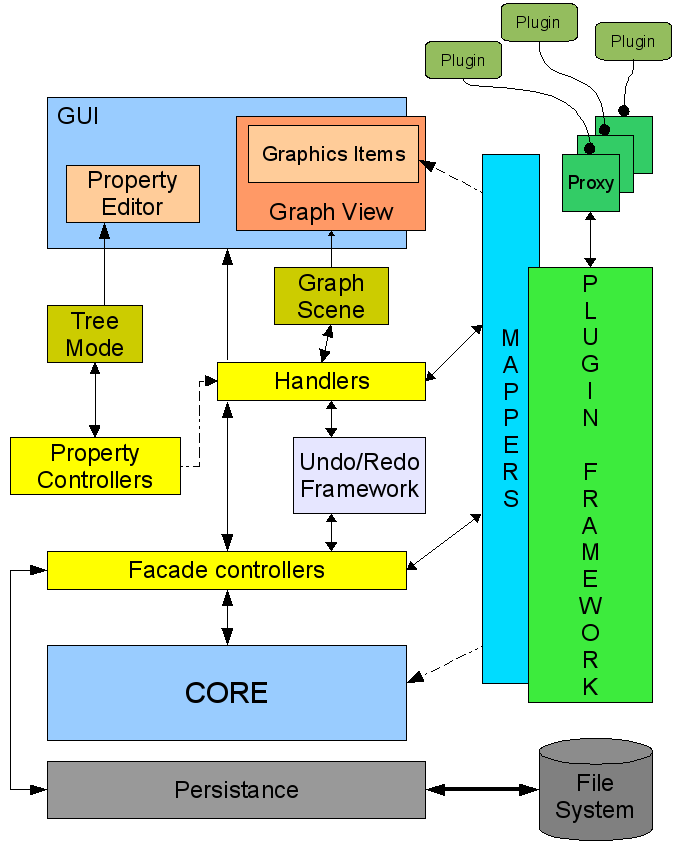
\includegraphics[width=8cm]{images/diagramma_componenti_vnetkit.png}
	\caption{Diagramma dei componenti di \visualnetkit{}}
	\label{figura:vn_componenti}
\end{figure}

In questa introduzione si vuole offrire un quadro generale (figura \ref{figura:vn_componenti}) della composizione architetturale nello stato attuale di \visualnetkit{}, in modo da rendere più facile la localizzazione degli elementi durante la loro trattazione.

\section{Architettura modulare basata su \plugin{}}
Si procederà dapprima all'analisi della struttura modulare del sistema che rappresenta anche il suo punto di forza per quanto riguarda la flessibilità e l'estensibilità. 

Può essere auspicabile che un software usato in ambito scientifico sia in possesso di funzionalità opzionali, vale a dire funzionalità che possono essere aggiunte o rimosse nel corso di una simulazione senza ostacoli di rilievo. Si pensi ad esempio a quanto possa essere utile ad un progettista osservare il comportamento di una rete con o senza un determinato servizio (ad esempio \emph{IPv6}) sulle macchine di cui è composta, o a quanto possa risultare comprensibile, per uno studente analizzare una topologia di rete malleabile che si presta a tutti i possibili test che intende effettuare.

L'utilizzo di un'architettura basata su \plugin{} dona grande flessibilità all'intero sistema ed in particolare offre ampia libertà di utilizzo agli utenti finali.

\subsubsection{Perché un sistema basato su \plugin{}?}
Durante le prime iterazioni e le prime fasi di testing sono emersi alcuni fattori di alto rischio. L'architettura era stata inizialmente concepita e realizzata sul concetto secondo cui tutti i requisiti dovevano essere assemblati staticamente nell'applicazione (come accade nei vari ambienti di configurazioni descritti nella sezione \ref{subsection:ccrc}).
Questa scelta prevedeva una lunghissima fase di sviluppo ed una continua ricerca dei requisiti e dei casi d'uso, che avrebbero potuto destabilizzare l'intero sistema. Inoltre, adottando questa tecnica non si sarebbe mai riusciti ad offrire una totale elasticità, ma piuttosto si sarebbe dovuti scendere a compromessi su cosa implementare e cosa no.

Analizzando nel dettaglio gli obiettivi, si è giunti alla conclusione che l'unica strada percorribile fosse quella che prevedeva la trasformazione dell'architettura monolitica in una modularizzata. Il core del sistema - senza alcun \plugin{} attivo - avrebbe offerto all'utente solamente la possibilità di creare una rete a livello topologico, ossia priva di caratteristiche proprie.

Questa nuova tecnica avrebbe da un lato offerto una sicura controllabilità dei fattori di rischio, restringendoli alla re-ingegnerizzazione del sistema per renderlo modulare, e dall'altro avrebbe reso \visualnetkit{} estremamente scalabile e gli avrebbe conferito una connotazione del tutto unica nel suo genere.

\subsection{Interazione tra sistema e \plugin{}}
Quando si sviluppa un'applicazione che si basa fortemente su \plugin{}, la cosa fondamentale è definire i confini dell'uno e dell'altro sistema. Sostanzialmente, nucleo e moduli devono essere ben descritti per non rischiare di imbattersi in fenomeni di sovrapposizione: questi due mondi devono cooperare ma non intralciarsi, né tantomeno svolgere le stesse mansioni.

Dopo un'attenta ed accurata fase di studio, si è arrivati a definire la linea di demarcazione tra il sistema e le estensioni. Queste ultime possono essere attivate sugli elementi di base della rete, offrendo una sorta di caratterizzazione più specifica. Su di un componente possono essere attivi contemporaneamente più \plugin{}, che di fatto donano una definizione ben precisa all'oggetto che li incapsula.
Se per esempio su un host si attivano \plugin{} quali DNS e HTTP, si può facilmente notare che il tipo di quell'oggetto non è altro che una semplice macchina virtuale che offre un servizio di DNS e che allo stesso tempo è un server Web.

In figura \ref{figura:uml_plugin_framework} è discritta in dettaglio la struttura del sotto sistema che permette ai moduli di colloquiare con il core dell'applicazione, e la definizione delle varie interfacce.
\begin{figure}[!htb]
	\centering
	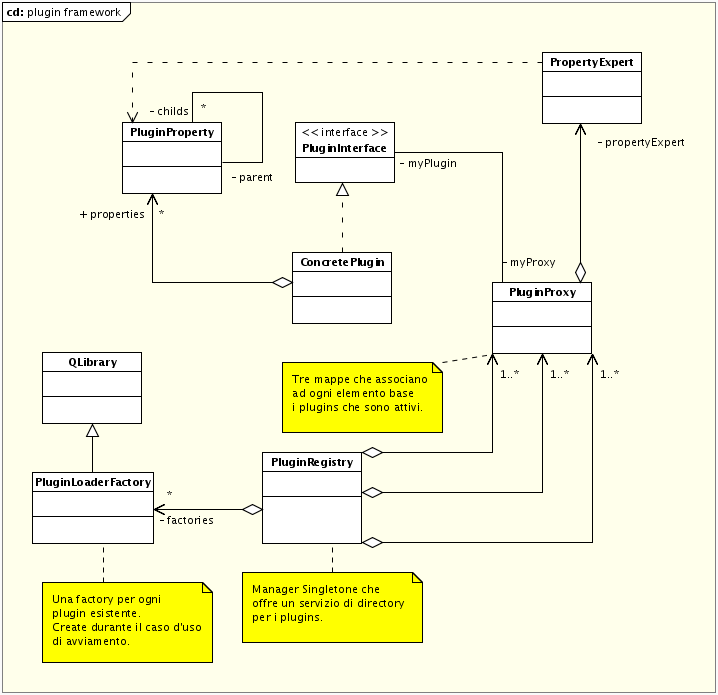
\includegraphics[width=12cm]{images/plugin_framework_uml.png}
	\caption{Diagramma delle classi del sotto sistema di gestione dei \plugin{}.}
	\label{figura:uml_plugin_framework}
\end{figure}
Come si può osservare dal diagramma delle classi, tutto ruota intorno all'entità singleton ``PluginRegistry''. Questo controller viene invocato dal sistema centrale nel caso d'uso d'avviamento per scandire il \fs{} e caricare in memoria i \plugin{} esistenti, validarli e creare per ognuno di questi il proprio \emph{loader factory}. Il PluginRegistry offre un servizio di directory, ossia è quel componente che mantiene traccia delle associazioni tra un \plugin{} e un elemento base.

In realtà il sistema non conosce direttamente l'instanza di un determinato modulo, ma conosce il suo \proxy{}, che introduce un livello di indirezione tra il core dell'applicazione e il \plugin{} stesso. La scelta di applicare il pattern \proxy{}\cite{SSA06} assicura un buon controllo d'accesso all'oggetto reale di cui è responsabile, e permette inoltre un colloquio trasparente verso il sistema. Si osservi ora la classe astratta pura PluginInterface:
\begin{lstlisting}
/**
 * PluginInterface.h
 */
class PluginInterface
{
public:
	virtual ~PluginInterface() {};

	virtual bool saveProperty(QString propUniqueId, QString propValue,
			QString *pluginAlertMsg = NULL) = 0;

	virtual QString getXMLResource() = 0;

	virtual QMap<QString, QString> getTemplates() = 0;
	
	virtual QList<PluginProperty*> getPluginProperties() = 0;

	virtual PluginProxy* getProxy() = 0;

	virtual void setProxy(PluginProxy* p) = 0;

	virtual void setGroupID(qint32 id) { Q_UNUSED(id) };
	virtual qint32 getGroupID() { return -1; };

	virtual QString getDefaultGraphisLabel() = 0;

	virtual QString getName() = 0;

	virtual bool init(QString laboratoryPath) = 0;
	
	virtual QString deleteProperty(QString propertyUniqueId) = 0;
	
	virtual QPair<PluginProperty*, QString> addProperty(
		QString propertyIdToAdd, QString parentPropertyUniqueId) = 0;
	
};

typedef PluginInterface* createPlugin_t();
typedef void destroyPlugin_t(PluginInterface*);
\end{lstlisting}

Trimite questa interfaccia un plugin può interagire con il sistema centrale. Ogni implementazione di un \plugin{} deve quindi riscrivere le funzioni descritte. Il modulo deve inoltre definire le factory di creazione e distruzione - righe $38$ e $39$. Queste due funzioni sono usate dalla classe LoaderFactory (che risolve i due simboli \textbf{createPlugin} e \textbf{destroyPlugin}) che permettono di creare nuove instanze di un determinato modulo.

Per avere informazioni aggiuntive su come creare un \plugin{}, si legga l'appendice a pagina \pageref{appendice_a}.

Ogni modulo è descritto da un proprio file di configurazione scritto in \xml{}, che deve necessariamente essere inserito all'interno del \emph{Qt Resource System}\footnote{Il sistema di risorse offerto da \qt{} consiste in un metodo per la memorizzazione di file binari all'interno dell'applicazione stessa (platform-indipendent). Questa è una tecnica molto utile quando l'applicazione ha sempre bisogno di determinati files e non si vuole correre il rischio di non possederli a runtime.}. All'interno di questo file vi sono strutturate le credenziali del \plugin{} come: il nome, la descrizione, gli autori, le dipendenze dagli altri \plugin{} ecc\ldots, ma anche un'accurata rappresentazione delle proprietà offerte all'elemento su cui verrà attivato il modulo.

Per facilitare questo processo, ogni \proxy{} è equipaggiato di una classe ``expert'' che si occupa della validazione e interrogazione del file \xml{} sopra citato, nonché della manipolazione delle properties memorizzate all'interno di una struttura ad alberi n-ari.

Il sotto sistema appena descritto offre la possibilità di estendere le funzionalità di \visualnetkit{}. I vari \plugin{} sono elementi passivi che vengono invocati dal sistema nei casi in cui: l'utente agisce su una property, l'utente inizializza un \plugin{}, ecc\ldots Tuttavia un modulo può anche interagire con il sistema stesso, ma solamente dopo che è stato invocato; questo avviene durante la fase di inizializzazione, quando il sistema invoca le funzioni di ``getXmlResource()'' e ``getDefaultGraphisLabel()'' per validare e scrivere una label nella vista del grafo della rete.

\subsection{La gestione avanzata delle properties dei \plugin{}}
La creazione di un \plugin{} in \visualnetkit{} è un'operazione che richiede uno stadio pre-implementativo che consiste nello stilare il file di configurazione in \xml{}. Questo, oltre a descrivere i meta-dati - come ad esempio il nome del modulo -, assolve il compito di descrittore strutturale delle properties che il \plugin{} offre.
Si osservi l'esempio riportato qui sotto:
\begin{lstlisting}[language=xml]
<plugin name="Test">
 
 <global type="vm" version="1.0" author="Alessio Di Fazio" dependencies="">
  <![CDATA[This is a test plugin.]]>
 </global>
 
 <properties>
  
  <property id="uniqueID-0" name="1" default_value="" min="1" max="1000">
   <![CDATA[Property 1]]>
   <childs>
    <property id="uniqueID-1" name="1-1" default_value="" min="1" max="2">
     <![CDATA[A sub property (1-1)]]>
     <childs>
      <property id="uniqueID-2" name="1-1-1"
                      default_value="" min="1" max="5">
       <![CDATA[A sub property (1-1-1)]]>
       <childs>
        <property id="uniqueID-3" name="1-1-1-1"
                      default_value="" min="0" max="3">
         <![CDATA[A sub property (1-1-1-1)]]>
         <childs />
       </childs>
      </property>
     </childs>
    </property> 
   </childs>
  </property>
  
  <property id="uniqueID-4" name="p-2" default_value="" min="0" max="3">
   <![CDATA[Property 2]]>
   <childs />
  </property>
  
 </properties>
 
</plugin>
\end{lstlisting}
è possibile osservare una prima parte che descrive alcune caratteristiche del modulo quali il tipo di elemento a cui questo può essere applicato, il numero di versione, l'autore, il nome del \plugin{} e le dipendenze.

Il tag ``properties'' è il più importante e contiene tutte le possibili proprietà offerte, nonché una descrizione a livello gerarchico di queste ultime. La rappresentazione di una property deve contenere un ID univoco, un nome, un valore di default qualora necessario, un valore di minimo e massimo che rappresentano la cardinalità e una descrizione libera\footnote{La descrizione di una property può contenere anche codice HTML per la formattazione del testo.}.

I valori ``min'' e ``max'' rappresentano gli attributi principali. Il primo può assumere valori pari a $0$ o $1$, mentre il massimo può contenere qualsiasi valore compreso tra $1$ e $65536$ (un intero senza segno a $16$ bit). Impostando un valore minimo pari a $1$, la property in questione viene creata insieme all'instanza del \plugin{}, ed insieme alla property ``padre'' se quest'ultima viene in futuro aggiunta dall'utente.

Il controllo durante le azioni di inserimento e la cancellazione delle properties è a carico del modulo, il quale è tenuto a verificare il valore della cardinalità attuale di una property prima di eliminarla. Come è facilmente intuibile, un \plugin{} non può autorizzare l'eliminazione di una proprietà - priva di altre copie - quando la cardinalità minima di quest'ultima è pari a $1$. Un discorso analogo può essere applicato all'attributo ``max''.

\section{Elementi architetturali}
Appurato il funzionamento e la logica che risiede dietro il framework dei \plugin{}, è possibile iniziare ad introdurre gli altri elementi architetturali che di fatto supportano e interagiscono l'un l'altro per soddisfare tutti i requisiti (funzionali e non) che il sistema offre.

Si inizierà ad analizzare gli elementi in figura \ref{figura:vn_componenti} con strategia \textbf{top-down} per quanto riguarda gli elementi che hanno una collocazione orizzontale, successivamente si analizzeranno i mappers ed in fine gli sforzi verranno convogliati nella descrizione del nuovo sistema che offre ai \plugin{} la possibilità di possedere un'alta dinamicità nelle proprietà che questi offrono.

\subsection{L'interfaccia utente}
Uno degli obiettivi principali di questo progetto è la realizzazione di un ambiente di configurazione di reti virtuali, che offra un'interfaccia grafica capace di fornire una vista intuitiva della rete virtuale.
Tale interfaccia, oltre a garantire un alto livello di ergonomia e usabilità, deve garantire buone capacità di adattamento al variare dei requisiti.

Sebbene la realizzazione di una interfaccia grafica possa dare l'impressione di essere un'attività semplice, durante tale periodo si incontrano molteplici difficoltà in quanto l'ambiente in esame si avvicina molto alla definizione di ``IDE''\footnote{Un \textit{integrated development environment} (IDE), in italiano ambiente integrato di sviluppo, è un software che aiuta i programmatori nello sviluppo del software.} orientato - nel nostro caso - allo sviluppo di reti virtuali.

La realizzazione dell'attuale interfaccia ha richiesto diversi cicli di sviluppo e raffinamento per ottenere un risultato apprezzabile ed intuitivo. Questa è composta da varie \emph{docks} - figura \ref{figura:vnetkit_graphics_view_1} - che al loro interno contengono vari sotto elementi come properties, zoom e miniatura del grafo, elementi attivi, struttura de Lab e un elemento centrale che rappresenta la scena che consente di disegnare la topologia di rete desiderata. L'ampio uso di grafica SVG fa si che all'utente arrivi subito un feedback positivo che incentiva lo stesso a sperimentare le caratteristiche offerte dall'ambiente in cui è inserito.

Il grafo non è altro che la vista della struttura del modello di dominio. Ogni elemento grafico (Hosts, Collision Domains, Links) è in relazione con un elemento di basso livello che incapsula le informazioni. Gli elementi grafici sono sostanzialmente degli oggetti che riflettono queste informazioni all'utente e gli consentono di interagire con gli elementi stessi.

L'esistenza del \emph{Graphics View Framework} offerto da \qt{}, ha reso minimi gli sforzi implementativi in quanto questo è fortemente basato sul pattern MVC, che consente di collegare uno stesso modello (la scena) a più viste come avviene per la scena e la \textit{dock} della miniatura - figura \ref{figura:vnetkit_graphics_view_1}.

\begin{figure}[!htb]
	\centering
	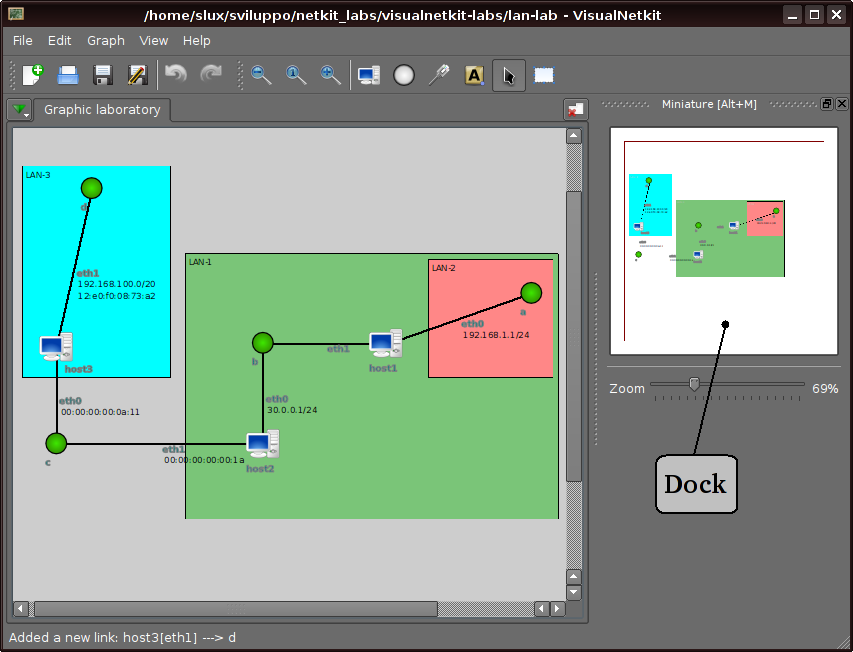
\includegraphics[width=12cm]{images/visualnetkit_graphics_view_1.png}
	\caption{Scena del grafo inserita in due viste differenti e difinizione di ``Dock''.}
	\label{figura:vnetkit_graphics_view_1}
\end{figure}

\subsubsection*{Dettagli implementativi}
L'interazione con l'utente è stata implementata seguendo i principi dell'\emph{event driven programming}, che rappresenta la base della programmazione delle interfacce grafiche. La programmazione guidata dagli eventi non considera i meccanismi standard di input (ad esempio la CLI - \emph{Command Line Interface}) ma basa il suo funzionamento sulla gestione degli eventi generati dall'utente, coma la pressione di un bottone o un click del mouse. 

L'insieme degli eventi di interesse vengono ricevuti da handlers che effettuano una prima validazione e inoltrano lo stesso evento agli strati di competenza, posti solitamente nei livelli più bassi dell'architettura.

\subsubsection*{Signals e Slots in \qt{}}
In \qt{} slot e segnali sono usati per la comunicazione asincrona tra oggetti.
Questo sistema fa in modo che oggetti di un certo tipo vengano avvertiti e siano in grado di comunicare con altri elementi, quando su di un oggetto si scatena un determinato evento. Per esempio, se un utente clicca un bottone \textbf{Close}, probabilmente si vorrebbe che il widget si chiuda chiamando la sua funzione ``close()''.

Un segnale viene emesso quando un particolare evento accade, uno slot è invece una funzione che se invocata, è responsabile di gestire un particolare segnale. Può però anche essere invocata in maniera sincrona da un qualche altro oggetto.
Tale meccanismo nasconde in realtà un sistema già noto con il nome di pattern \textit{Observer}. L'unica differenza risiede nelle chiamate asincrone che i signal effettuano allo slot di loro competenza, senza aspettare una risposta. Infatti, ogni slot è definito con un tipo di ritorno ``void'', e l'unico metodo che permette di effettuare modifiche sui dati è tramite effetti collaterali sull'elemento passato come puntatore. In figura \ref{figura:qt_signals_slots} è mostrato un esempio d'uso di Signals e Slots.

\begin{figure}[!htb]
	\centering
	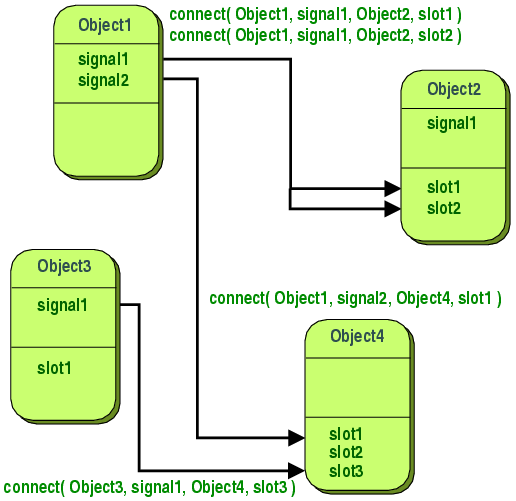
\includegraphics[width=8cm]{images/signals_slots.png}
	\caption{Schema d'uso di Signals e Slots.}
	\label{figura:qt_signals_slots}
\end{figure}

\subsubsection*{L'editor testuale}
\visualnetkit{} non offre solamente la possibilità di disegnare la rete di calcolatori e caratterizzarla tramite l'applicazione dei moduli. Durante la realizzazione di un Lab è possibile che l'utente voglia autonomamente applicare modifiche ai files di configurazione che l'ambiente produce.

Per questo motivo \visualnetkit{} include al suo interno un editor di testo potente che offre un elevato numero di regole per il \emph{Syntax Highlighting}, come mostrato in figura \ref{figura:vn_text}. Ogni singolo editor offre la possibilità di annullare le modifiche (Undo e Redo) e salvare il testo, dando la possibilità di creare una copia di backup.

\begin{figure}[!htb]
	\centering
	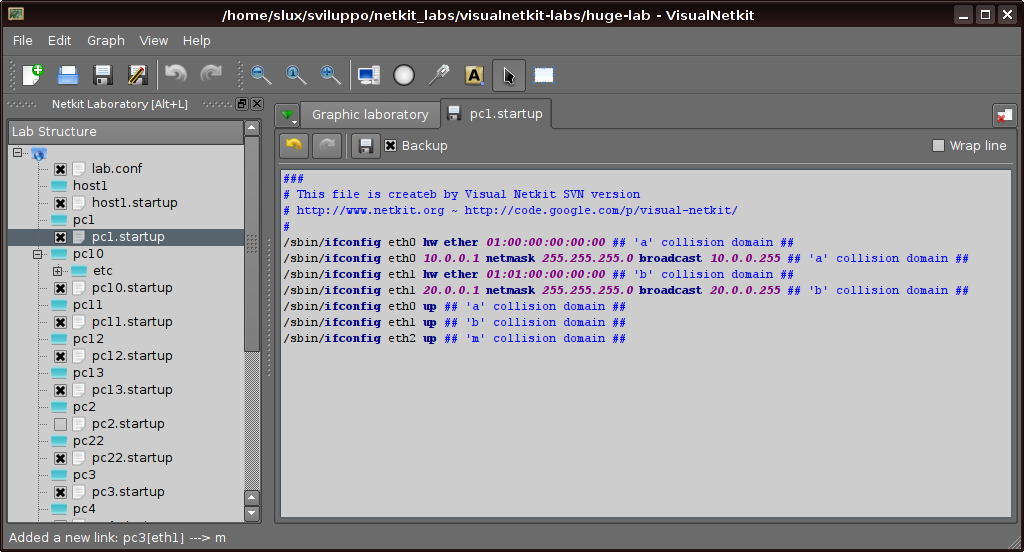
\includegraphics[width=12cm]{images/visualnetkit_editor.png}
	\caption{L'editor testuale di \visualnetkit{}}
	\label{figura:vn_text}
\end{figure}

\subsection{Elementi del dominio}
Il kernel di questo progetto è il primo componente che è stato sviluppato ed anche il più importante. In esso sono contenuti tutti gli oggetti elementari su cui si basa la topologia di rete che l'utente vuol creare. Le classi rappresentano elementi della realtà di interesse come le virtual machine, i collision domain, le hardware interface e anche l'intero laboratorio.

Come si nota dal diagramma delle classi presente in figura \ref{figura:uml_package_core}, questo package ha una struttura molto semplice, ma allo stesso tempo riesce a descrivere qualsiasi topologia di rete virtuale. Infatti, un laboratorio è composto da un insieme di oggetti VirtualMachine e CollisionDomain contenuti all'interno di due Mappe ordinate per nome.

La giunzione tra questi ultimi due elementi è occupata dalla classe HardwareInterface che funge da collante di riferimento tra l'host virtuale, ed i vari domini di collisione a cui è collegato.
Grazie a questa semplice struttura \visualnetkit{} nasce da una parte come ambiente per la creazione di reti virtuali da emulare con \netkit{}, ma è dall'altra potenzialmente in grado di essere riadattato in modo da poter produrre configurazioni per altri sistemi di emulazione.

\begin{figure}[!htb]
	\centering
	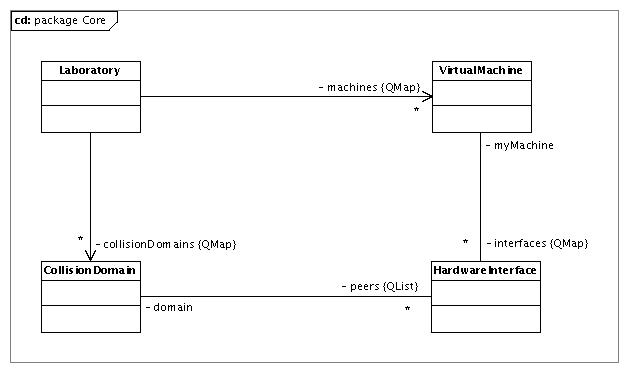
\includegraphics[width=12cm]{images/uml_package_core.png}
	\caption{Diagramma delle classi del package Core.}
	\label{figura:uml_package_core}
\end{figure}

Come vedremo più avanti, gli oggetti di tipo HardwareInterface saranno rappresentati da dei Links visualizzati come linee \emph{SVG} all'interno della scena grafica.

\subsection{La gestione degli eventi}
Come in tutte le applicazioni software, ogni oggetto ha bisogno di essere ``gestito'' nel contesto dell'applicazione stessa.
La funzione di amministrazione e controllo del singolo oggetto - in applicazioni realizzate a regola d'arte -, viene demandata ad altri oggetti tipicamente più leggeri ma non per questo meno complessi, detti \emph{handler}.

Le funzioni di controller sono state realizzate seguendo le linee guida del pattern \emph{Controller}\cite{AUPL04} ed assegnando le responsabilità del controllo e compiti dell'oggetto interessato. In \visualnetkit{} esistono vari tipi di \emph{handlers}:
\begin{itemize}
\item \emph{Facade Controllers};
\item \emph{Use Case Controllers};
\item \emph{Mappers} - macro elementi che disaccoppiano vista e dominio;
\item \emph{Property Controllers}.
\end{itemize}

I \emph{Facade Controllers} vengono utilizzati per raccogliere le richieste che provengono dai livelli più alti - in particolare dagli \emph{Use Case Controllers} - quando c'è bisogno di un accecesso a basso livello che comporta un qualche tipo di cambiamento delle strutture del Dominio.

Gli \emph{Use Case Controller}\footnote{Nella figura \ref{figura:vn_componenti} sono indicati come \emph{Handlers} generici.} sono posti in strati medio-alti dell'architettura e sono i primi oggetti che ricevono i segnali provenienti dall'interfaccia grafica. Questi effettuano una prima validazione dell'atto svolto e, se non vi sono errori, inoltrano la richiesta agli oggetti più bassi, in particolare ai \emph{Facade Controllers} e, in qualche caso anche agli oggetti \emph{Mappers}.


\subsection{Interazione tra Utente e Proprietà degli Elementi}
Ogni elemento del dominio incapsula alcune proprietà di base. Queste, oltre a caratterizzare i vari oggetti, servono anche per descrivere una certa realtà di interesse espressa dall'utente. Ciò significa che è proprio il cliente finale che vuole avere la facoltà di cambiare questi attributi in ogni momento.

In \visualnetkit{}, oltre alle proprietà offerte dagli oggetti del dominio (ad esempio il nome di una \virtualmachine{}), per la natura modulare del sistema, è possibile che per un oggetto base vi siano collegati alcuni \plugin{} che offrono proprietà aggiuntive.
La gestione di queste è demandata ad oggetti - di tipo \emph{Use Case Controller} - che sono responsabili di renderizzare i dati e ricevere le modifiche che l'utente desidera (figura \ref{figura:properties_uml1}).

È possibile osservare come questi oggetti vengono dinamicamente inseriti come handlers degli elementi che rappresentano i dati delle properties, poiché la natura delle entità che l'utente può selezionare è eterogenea: ogni tipologia di elemento possiede il suo \emph{Property Controller}.

\subsection{Gestione degli annullamenti: l'Undo Framework}
Per l'implementazione delle funzionalità di undo e di redo delle azioni svolte è stato utilizzato un potente framework offerto da \qt{}. Questo sistema ha permesso, in fase realizzativa, di tralasciare molti dei dettagli implementativi e dirigere l'attenzione verso problematiche come la consistenza dei dati. Infatti, sebbene le operazioni di undo o redo siano atomiche, esse interagiscono con lo strato dei \emph{Facade Controllers} e quindi indirettamente anche con gli oggetti del Dominio.

\subsubsection*{L'Undo Framework in \qt{}}
Il \emph{Qt Undo Framework} è un'implementazione del pattern \emph{Command}\cite{AUPL04} per l'attuazione di funzionalità di undo/redo nelle applicazioni.
Il pattern \emph{Command} è basato sul concetto che tutte le funzioni di editing in un'applicazione sono realizzate con la creazione di instanze di elementi command. Analizzando l'esempio di un editor di testo, gli oggetti command applicano le modifiche al documento e sono memorizzati in uno stack dei comandi.

Un \emph{QUndoCommand} rappresenta un singolo atto di editing all'interno del documento come, ad esempio, l'inserimento o l'eliminazione di blocchi di testo. Un comando può apportare cambiamenti al documento con azioni di \emph{redo()} o di \emph{undo()}.

Inoltre, ogni comando è capace di annullare i cambiamenti da lui apportati e come riportare il documento allo stato precedente. Finché l'applicazione utilizza solo oggetti command per cambiare lo stato del documento, è possibile annullare una sequenza di comandi attraversando lo stack verso, disfacendo ciascun comando presente. È anche possibile ripetere una sequenza di comandi percorrendo la pila all'inverso.

La flessibilità offerta da questo strumento è tale da poter essere applicata ad ogni tipo di situazione. Viene ora analizzato un esempio un po' più realistico e complesso.

Nel framework ogni azione che l'utente vuole poter annullare è implementata in una classe che estende \emph{QUndoCommand}. Per ogni azione effettuata viene creato un apposito command che andrà inserito nel \emph{QUndoStack} di riferimento. Appena l'oggetto prende posto all'interno dello stack, il framework provvede ad invocare la sua funzione di redo per completare e/o effettuare l'azione richiesta.

L'esempio riportato implementa un semplice diagramma grafico, è pertanto possibile eliminare e aggiungere elementi e muoverli tramite \emph{drag\&{}drop}. Ognuna di queste azioni possiede il corrispondente undo-command, che permette eventualmente all'utente di tornare sui suoi passi.
In figura \ref{figura:qt_undo} è mostrato come un \emph{QUndoStack} può essere mostrato graficamente all'interno di un \emph{QUndoView}, dove ogni riga presente rappresenta un singolo Command.

\begin{figure}[!htb]
	\centering
	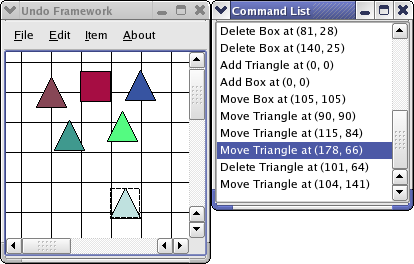
\includegraphics[width=10cm]{images/undoframeworkexample.png}
	\caption{Un esempio avanzato dell'Undo Framework offerto da \qt{}.}
	\label{figura:qt_undo}
\end{figure}

\subsection{L'accesso al \fs{}}
Lo strato di persistenza dei dati nel complesso di ogni applicazione software gioca un ruolo fondamentale. Generalmente posto nello strato più basso del sistema, questo elemento architetturale ha il duplice scopo di interagire con il \fs{} per salvare i dati inerenti alle varie configurazioni dell'applicazione e dei laboratori creati, nonché esportare questi ultimi in un formato accettato e riconosciuto dall'ambiente di emulazione desiderato.

Uno dei problemi riscontrati in fase di progettazione è stato come strutturare le informazioni che dovevano essere salvate. Da una parte occorreva memorizzare lo stato del laboratorio creato - in particolare lo stato del grafo della rete -, mentre dall'altra era necessario trovare un buon sistema per poter esportare il laboratorio in modo da essere poi eseguito correttamente dal sistema di emulazione su cui quest'ambiente si basa\footnote{Ribadiamo il concetto che \visualnetkit{} nasce come ambiente per creazione di lab per \netkit{}, ma questo non vincola il tool ad un eventuale adattamento in favore di un qualsiasi altro sistema di emulazione.}.

Ad esempio, se un utente desidera salvare un Lab per poi riaprirlo, dev'essere possibile memorizzare meta-dati sugli elementi presenti nella scena grafica, che potrebbero essere la posizione degli oggetti stessi o delle etichette, ed eventuali informazioni inerenti ai \plugin{}.

Si è deciso di procedere, quindi, con la registrazione delle meta-informazioni su di un file in formato \xml{} nominato \emph{lab.xml}, posto nella root directory del laboratorio.
Il fatto di salvare i meta-dati in un file separato rende il lab prodotto standard e auto descritto da un singolo file di configurazione esterno.
Un tag principale ``scene'' rappresenta alcune informazioni sulla scena grafica, come ad esempio la dimensione. Internamente a questo vi sono tags di gruppo che descrivono i vari componenti grafici come links, aree, virtual machines e collision domains. Ad ognuno di questi sono associate informazioni extra che descrivono meta-dati aggiuntivi, quando previsto.

La porzione del sistema che esporta la struttura del laboratorio su \fs{}, compie quattro fasi:
\begin{description}
\item[Fase 1] questo stadio iniziale è adibito alla creazione della struttura base delle directories. In particolare, per ogni \virtualmachine{} presente nel Lab creato viene prodotta una directory con il nome dell'host;

\item[Fase 2] è il momento della creazione del file \emph{lab.conf} che contiene la struttura fondamentale della rete a livello topologico, riconosciuta da \netkit{};

\item[Fase 3] questa fase è riservata al salvataggio dei file di ``sturtup'' delle macchine presenti\footnote{In \netkit{} ogni host virtuale che viene avviato può operare azioni di post-start grazie all'esecuzione del file \emph{.startup} che rappresenta una precisa macchina virtuale.};

\item[Fase 4] l'ultimo step permette ad ogni plugin attivo di offrire porzioni (o la totalità) di file di configurazioni che descrivono i propri settaggi.
\end{description}

\subsubsection*{Template Engine in \visualnetkit{}}
Nelle fasi due, tre e quattro si è parlato della creazione dei file di configurazione. Sia i \plugin{} che l'applicazione stessa utilizzano un sistema di \emph{mark-up} per la costruzione dei vari templates, i quali andranno poi scritti dallo strato di persistenza all'interno dei files. Questi templates possiedono una struttura interna che prevede la sostituzione localizzata di alcune parti. Si prenda in esame il templete utilizzato per creare il file ``lab.conf'':
\begin{lstlisting}[language=csh]
###
# This file is createb by Visual Netkit <VISUAL_NETKIT_VERSION> version
# http://www.netkit.org ~ http://code.google.com/p/visual-netkit/
#

LAB_DESCRIPTION="<DESCRIPTION>"
LAB_VERSION="<VERSION>"
LAB_AUTHOR="<AUTHOR>"
LAB_EMAIL="<EMAIL>"
LAB_WEB="<WEB>"

<TOPOLOGY><HOST>[<ETH_NUMBER>]="<COLLISION_DOMAIN_NAME>"</TOPOLOGY>
\end{lstlisting}
Il Template Engine interno all'applicazione viene invocato passando il riferimento (basato sul resource system di \qt{}) ad un template file. Questo viene dapprima caricato in memoria e successivamente, vengono effettuare alcune sostituzioni di base come quella del \emph{mark-up}\\
\texttt{<VISUAL\_{}NETKIT\_{}VERSION>}, che viene sostituito dalla corrente versione del tool.

L'elemento che invoca il caricamento di un template riceve quindi il contenuto del file desiderato. In seguito vengono effettuate le altre sostituzioni tramite l'ausilio di espressioni regolari talvolta complesse.

Si osservi la riga $12$: l'oggetto incaricato di salvare il file ``lab.conf'' ha la mansione di completare la struttura del file di configurazione inserendo la descrizione, la versione, l'autore, l'indirizzo email e il sito web del lab corrente, ed in secondo luogo andrà a costruire successivamente la topologia dell'intera rete, iterando tra i \emph{tag} \texttt{<TOPOLOGY></TOPOLOGY>}.

In questo modo si riesce a creare un file di configurazione corretto e ben formattato come quello proposto qui sotto, che descrive la topologia di rete presente in figura \ref{figura:vnetkit_graphics_view_1}.
\begin{lstlisting}[language=csh]
###
# This file is createb by Visual Netkit 1.1 version
# http://www.netkit.org ~ http://code.google.com/p/visual-netkit/
#

LAB_DESCRIPTION="A simple laboratory"
LAB_VERSION="1.0"
LAB_AUTHOR="Alessio Di Fazio"
LAB_EMAIL="slux83@gmail.com"
LAB_WEB="http://code.google.com/p/visual-netkit/"

host1[0]="a"
host1[1]="b"

host2[0]="b"
host2[1]="c"

host3[0]="c"
host3[1]="d"
\end{lstlisting}

È importante notare come il template dell'esempio appena citato risulti totalmente indipendente dal motore di emulazione utilizzato, ed è dunque facilmente rimodellizzabile al fine di essere impegnato con emulatori differenti.

Nel caso in cui un emulatore richiedesse una sintassi particolare per le varie macchine virtuali, come ad esempio VNUML, basterebbe creare un semplice \plugin{} che offra uno specifico template ed aggiungere questo \plugin{} ai vari host virtuali presenti nella topologia di rete.

\subsection{Controllers tra Dominio e Vista}
Un ulteriore elemento architetturale che spicca nella figura \ref{figura:vn_componenti} è il componente \emph{Mapper}. Questo package è composto da varie classi \emph{singleton}, predisposte al ruolo di mappare gli oggetti della vista in quelli del dominio, e viceversa. Da ciò deriva la verticalità che assume tale componente all'interno del diagramma.

\begin{figure}[!htb]
	\centering
	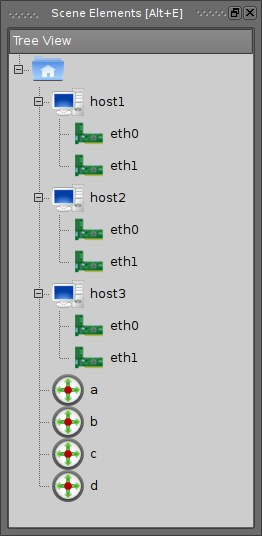
\includegraphics[width=4cm]{images/visualnetkit_tree_elements.png}
	\caption{Albero degli elementi presenti sulla scena.}
	\label{figura:scene_elements}
\end{figure}

Ogni tipologia di oggetti del dominio possiede un proprio mapper di riferimento. Questo è ciò che accade per una \virtualmachine{} che deve essere associata al corrispettivo elemento grafico. Tale scenario è reso possibile grazie al mapper per le macchine virtuali (\emph{VmMapper}).

Questi ``controllers'' inoltre, hanno il compito di disaccoppiare gli oggetti della vista con quelli del dominio, inserendo un ulteriore livello di indirezione. Tale soluzione è stata studiata per ovviare al noto problema che il pattern MVC introduce, ossia il forte accoppiamento tra la vista e il modello.

In questo contenitore possiamo individuare diversi tipi di mappers. Oltre a quelli utilizzati come controllers per gli oggetti del dominio, vi sono elementi - \emph{ad esempio SceneTreeMapper} - che si occupano principalmente di mantenere allineato lo stato degli elementi del dominio con una determinata porzione dell'interfaccia utente, in questo caso l'albero degli elementi grafici (figura \ref{figura:scene_elements}).

\section{Strumenti di supporto allo sviluppo}
Durante tutto il lavoro sono stati utilizzati molteplici strumenti che hanno contribuito alla realizzazione del prodotto.

\subsection{Il framework \qt{}}
\qt{} è un \emph{framework applicativo multi-piattaforma} (figura \ref{figura:qtframework}) per la realizzazione di software desktop ed \emph{embedded}, sviluppato da \emph{Nokia-Trolltech} e distribuito in versioni per uso commerciale e open source, quest'ultima sotto licenza \emph{GPL-3}. \qt{} include una documentazione (\textbf{A}pplication \textbf{P}rogram \textbf{I}nterface) molto intuitiva ed un ricco insieme di classi \cpp{}, strumenti integrati per lo sviluppo e l'internazionalizzazione delle GUI, e il supporto per lo sviluppo in Java e \cpp{}.

Sono inoltre presenti svariati sistemi di binding per altri linguaggi di scripting quali QtPerl, QtPython, QtRuby, ecc\ldots

\begin{figure}[hbt]
	\centering
	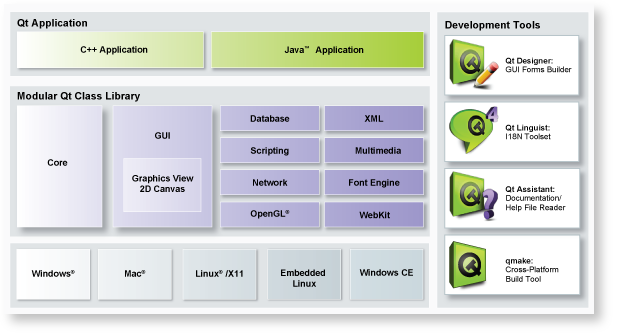
\includegraphics[width=12cm]{images/qtframework.png}
	\caption{Panoramica degli elementi presenti nel framework \qt{}.}
	\label{figura:qtframework}
\end{figure}

La modularità delle librerie \qt{} fornisce un ricco insieme di estensioni per la costruzione di applicazioni, integrando tutte le funzionalità necessarie per la creazione di software avanzati e multi-piattaforma.

Il framework equipaggia inoltre strumenti di sviluppo integrato per la realizzazione assistita di interfacce grafiche, traduzione e internazionalizzazione, documentazione e realizzazioni. Ossi i \emph{Development Tools}.

\subsubsection{Qt Designer}
\emph{Qt Designer} è un potente strumento per la costruzione di GUI e form con layout nativo e multi-piattaforma. Questo consente la rapida progettazione e realizzazione di ``widgets'' e finestre di dialogo, utilizzando le stesse tecniche di programmazione e mantenendo il tutto disaccoppiato dall'implementazione dal sistema. Le form create con \emph{Qt Designer} godono di piena funzionalità e possono essere visualizzate in anteprima in modo da garantire che il loro impatto visivo rifletta esattamente le aspettative del programmatore.

Una volta creato il widget con l'ausilio del tool in questione, viene prodotto un file con estensione \texttt{.ui}, che al suo interno contiene una struttura basata su \xml{}. All'interno dell'applicazione, la form dovrà essere implementata collegando questo file (\textbf{U}ser \textbf{I}nterface) all'oggetto che si vuole utilizzare nel sistema in questione.

Esistono vari metodi per collegare un file UI ad una classe della nostra applicazione. Quello utilizzato durante l'intero lavoro prende il nome di ``Multiple Inheritance Approach'' che consiste nell'inserire la form creata tramite \emph{Qt Designer} all'interno del file di progetto del sistema. Il pre-compilatore (uic - User Interface Compiler) si preoccuperà di trasformare il file \xml{} in un header \cpp{} da poter utilizzare nella classe concreta del widget. Si osservi l'esempio riportato di seguito:
\begin{lstlisting}
/**
 * ui_calculatorform.h e' l'header creato
 * tramite il pre-compilatore `uic'
 */
#include "ui_calculatorform.h"

/**
 * Implementazione del widget creato con QtDesigner
 */
class CalculatorForm : public QWidget, private Ui::CalculatorForm
{
    Q_OBJECT
public:
    CalculatorForm(QWidget *parent = NULL);

private slots:
    void on_inputSpinBox1_valueChanged(int value);
    void on_inputSpinBox2_valueChanged(int value);
};
\end{lstlisting}
La classe concreta \emph{CalculatorForm} deve estendere \emph{Ui::CalculatorForm} privatamente per assicurare che l'oggetto sia un rappresentante del widget creato con \emph{Qt Designer}.

A differenza di altri strumenti per la creazione di interfacce grafiche, \emph{Qt Designer} mette a disposizione dell'utente una quantità di strumenti (figura \ref{figura:qtdesigner}) che permettono di muovere e scalare gli elementi nell'interfaccia in modo automatico, offrendo quindi layouts auto-adattabili. Ne consegue che le interfacce sono sia funzionali che native, e si adattano comodamente all'ambiente operativo ed alle preferenze dell'utente.

\begin{figure}[!htb]
	\centering
	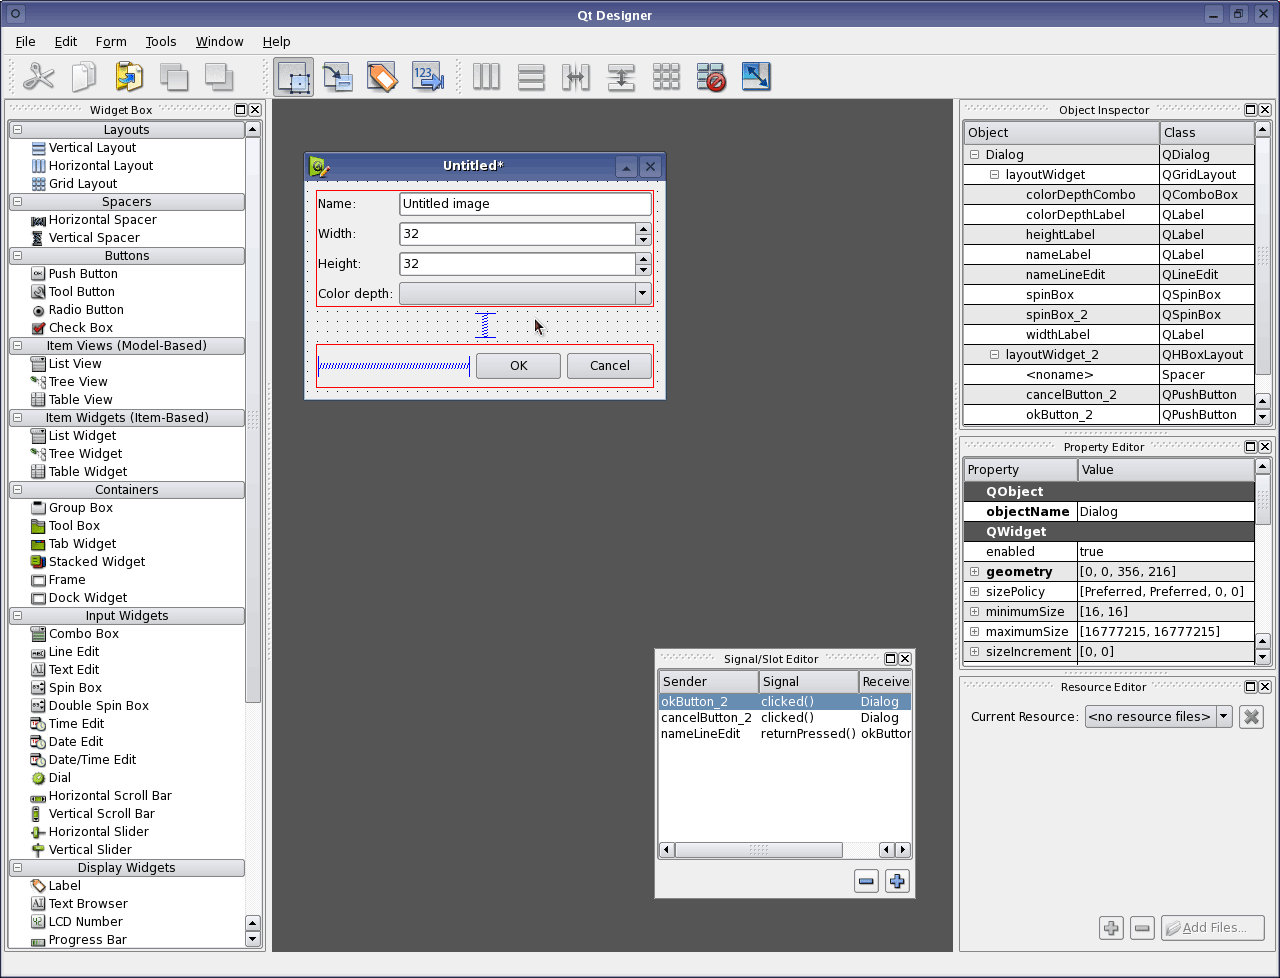
\includegraphics[width=12cm]{images/qtdesigner.png}
	\caption{Un esempio di utilizzo di \emph{Qt Designer}.}
	\label{figura:qtdesigner}
\end{figure}


\subsubsection{Qt Linguistic}
\emph{Qt Linguistic} fornisce una serie di strumenti che velocizzano la traduzione e l'internazionalizzazione delle applicazioni (\emph{i18n}). \qt{} offre anche il supporto simultaneo a più lingue e sistemi di scrittura, il tutto con un solo albero dei sorgenti ed un solo codice binario.

Il tool fornisce inoltre un'interfaccia che riduce i tempi del processo di traduzione della GUI, raccogliendo tutto il testo presente nelle UI che verrà mostrato all'utente finale in una finestra separata, per facilitarne la traduzione. Quando il testo è tradotto, il programma procede automaticamente alla prossima UI, fino a quando saranno completate tutte. Questo consente una più veloce e più accurata traduzione, offrendo alle applicazioni un supporto completo all'internalizzazione.

\subsubsection{Qt Assistant}
La maggiorparte delle applicazioni necessita di documentazione on-line o di un file di aiuto. \emph{Qt Assistant} è un lettore di documentazioni configurabile (figura \ref{figura:qtassistant}) che può essere facilmente personalizzato e ridistribuito con le singole applicazioni create, e che funziona in modo simile ad un browser web presentando la documentazione come una raccolta di pagine e collegamenti ipertestuali. 
\begin{figure}[!htb]
	\centering
	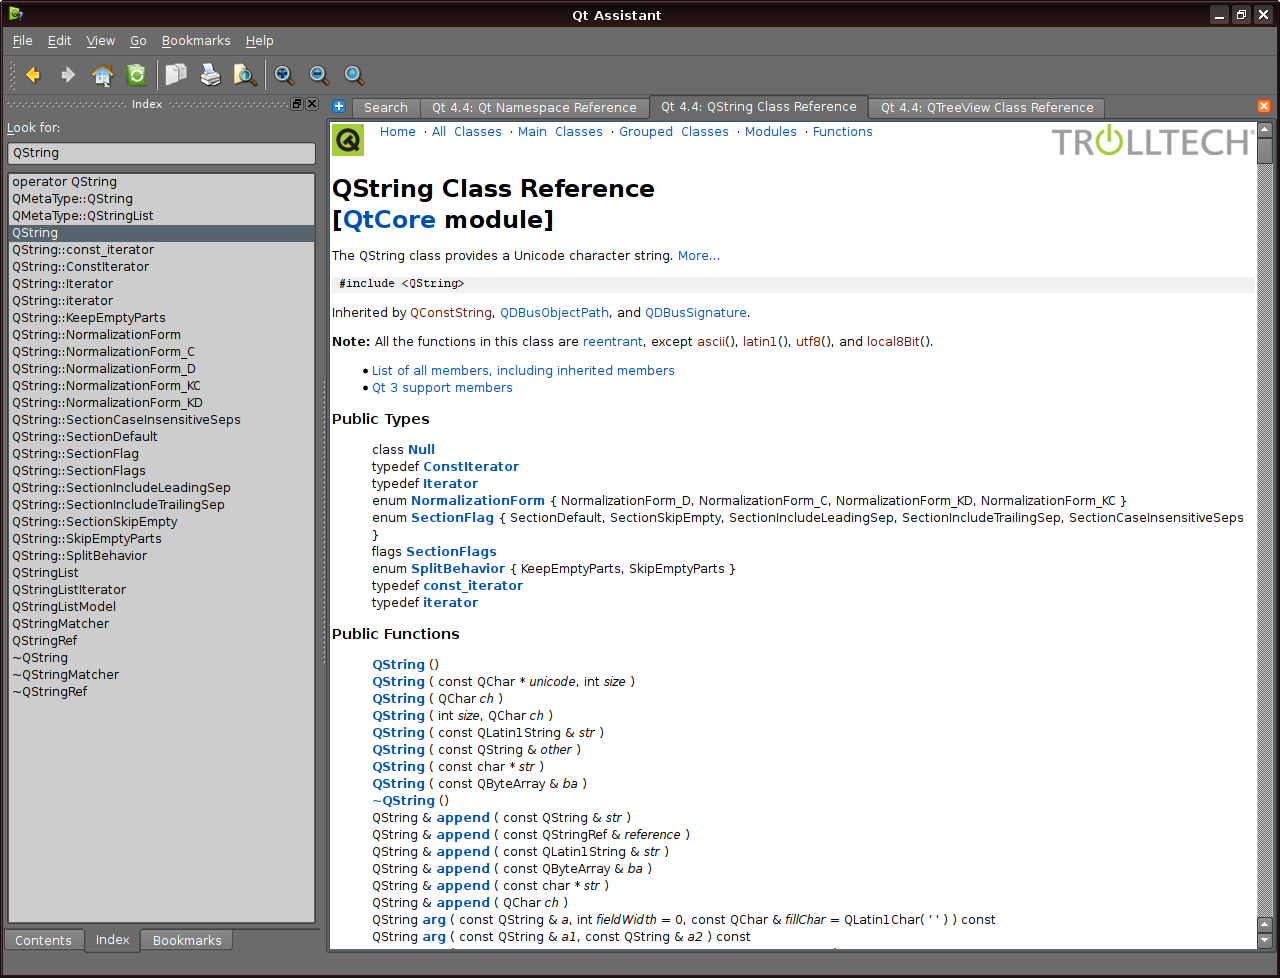
\includegraphics[width=12cm]{images/qtassistant.png}
	\caption{\emph{Qt Assistant}.}
	\label{figura:qtassistant}
\end{figure}
Questo riconosce pagine con segnalibri e presenta i pulsanti standard ``precedente'' e ``successivo'' nella barra degli strumenti per la navigazione tra le pagine visitate. \emph{Qt Assistant} utilizza il l'insieme della documentazione offerta dalle librerie \qt{} nei formati \emph{rich text} e HTML per la visualizzazione delle pagine. Ciò significa che redattori e tecnici non hanno bisogno di software ad-hoc per creare la propria documentazione, ma possono utilizzare gli strumenti come \emph{Doxygen} per scrivere i meta-dati direttamente nei sorgenti.

Il tool fornisce anche un veloce strumento di ricerca per accedere rapidamente all'argomento di interesse. I documenti rinvenuti nel corso di un'indagine vengono riportati in ordine di rilevanza, ed ogni occorrenza della parola chiave all'interno della documentazione viene evidenziata.

\subsubsection{QMake}
\emph{QMake} è uno strumento multi-piattaforma che semplifica il processo di costruzione dei progetti \qt{} su diversi sistemi. A seconda del sistema operativo in cui ci si trovi, \emph{QMake} genera i vari  \emph{Makefiles} in modo da essere compatibili con la piattaforma utilizzata.

\emph{QMake} genera un Makefile sulla base delle informazioni presenti all'interno del file di progetto. Questi ultimi vengono creati dallo sviluppatore e sono molto semplici; un tipico esempio è riportato sotto:

\begin{lstlisting}[language=csh]
#############################################
#
# Example of .pro file
#
#############################################

TEMPLATE  = app
TARGET    = test
LANGUAGE  = C++
CONFIG   += console debug

QT += core \
      gui

HEADERS   = stable.h \
            mydialog.h \
            myobject.h
SOURCES   = main.cpp \
            mydialog.cpp \
            myobject.cpp \
            util.cpp
FORMS     = mydialog.ui
\end{lstlisting}

\subsection{Altri strumenti secondari}

\subsubsection{Plugin Qt per Eclipse}
L'integrazione di \qt{} in \emph{Eclipse} consente ai programmatori di creare le applicazioni in modo veloce. I punti di forza di questo potente \plugin{} sono l'integrazione con i principali strumenti \qt{} precedentemente descritti, il notevole supporto nella creazione dei file di progetto, il completamento automatico durante la digitazione, e molti altri. Il potente debugger e l'ambiente che l'IDE offre in generale rendono questo strumento uno dei migliori editor per lo sviluppo di applicazioni \qt{}.
Per gli sviluppatori \emph{Java} e \cpp{} questo modulo - che estende le funzionalità dei \plugin{} base di \emph{Eclipse} - al momento attuale risulta la soluzione migliore tra tutte quelle testate.

\subsubsection{Umbrello UML Modeller}
\textit{Umbrello UML Modeller} - figura \ref{figura:umbrello_example} - è uno strumento per la realizzazione di diagrammi UML che si è rivelato essere di grande aiuto nel processo di sviluppo del software, specialmente durante le fasi di analisi e progettazione, in cui la creazione di \textit{diagrammi delle classi}, \textit{dei casi d'uso} e dei \textit{diagrammi di interazione} era spesso indispensabile. Umbrello ha contribuito a rendere il progetto chiaro soprattutto per quanto riguarda la documentazione delle scelte progettuali tra le parti interessate.

\begin{figure}[!htb]
	\centering
	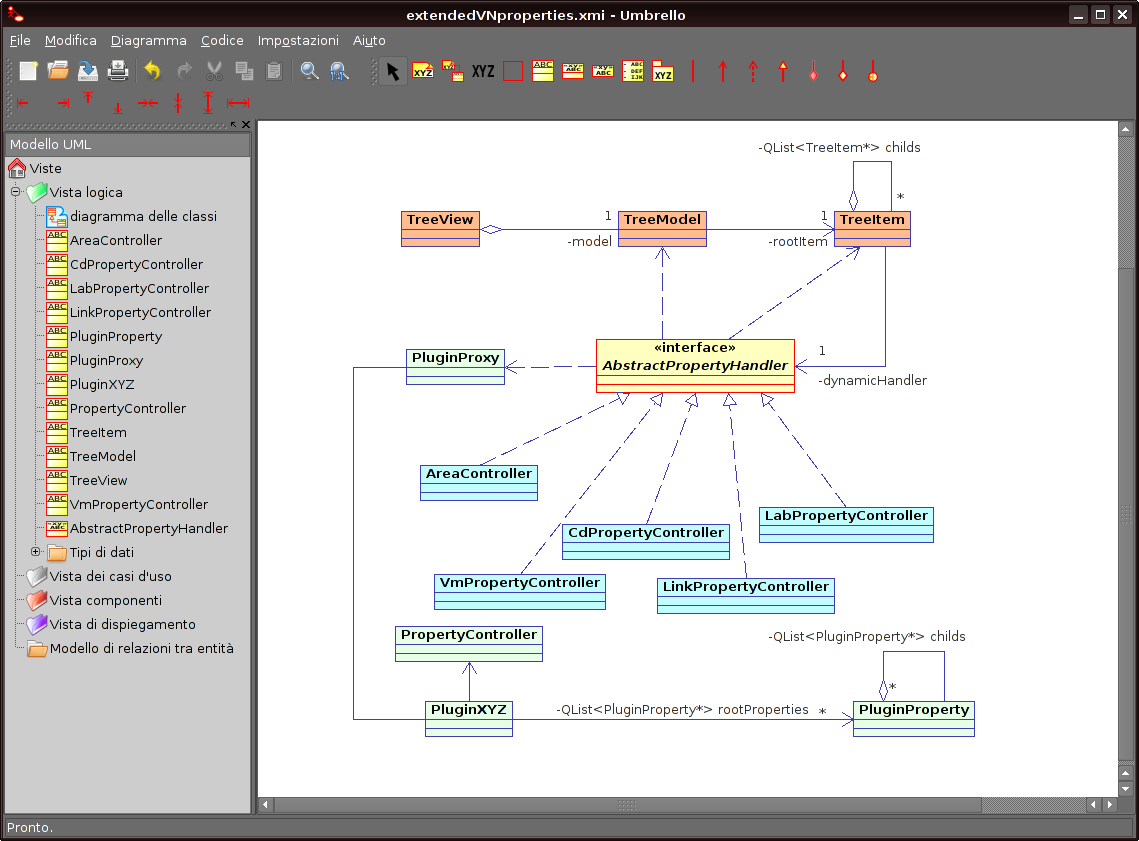
\includegraphics[width=10cm]{images/umbrello.png}
	\caption{Un esempio d'uso del tool \emph{Umbrello}.}
	\label{figura:umbrello_example}
\end{figure}

\subsubsection{SVN e Google Code}
A supporto dell'intero sviluppo si sono utilizzati gli strumenti per la gestione del codice \textit{SVN} e \textit{Google Code}.
In particolare, SVN è stato usato come strumento principale per gestire la continua evoluzione dei documenti relativi al progetto, come il codice sorgente del software, i disegni tecnici ed i diagrammi, la documentazione, e altre informazioni importanti su cui si è lavorato.

Nella maggiorparte dei progetti di sviluppo software, più sviluppatori lavorano in parallelo sullo stesso codice. Se due sviluppatori tentano di modificare lo stesso file contemporaneamente, in assenza di un metodo di gestione degli accessi, essi possono facilmente sovrascrivere o perdere le modifiche effettuate contestualmente.
La maggior parte dei sistemi di controllo versione possono risolvere questo problema in due diversi modi. Alcuni di questi prevengono i problemi dovuti ad accessi simultanei semplicemente bloccando i file (mediante l'utilizzo di un \textit{lock}), cosicché solamente uno sviluppatore alla volta riceve i permessi di accesso in scrittura alla copia di quel file, contenuta nel \textit{repository} centrale. Altri, come CVS, permettono a più sviluppatori di modificare lo stesso file contemporaneamente e forniscono gli strumenti per combinare in seguito le modifiche, tramite operazioni di \emph{merge}.

\emph{Subversion} (noto anche come SVN) è un sistema di controllo versione progettato da \textit{CollabNet Inc.} nel $2000$ con lo scopo di essere il naturale successore di CVS, oramai considerato superato.

\textit{Google Code}, ed in particolare la sezione \textit{Project Hosting}, non è stato per questo progetto solo il repository dedicato all'SVN, ma ha messo a disposizione dei programmatori una serie di strumenti tra cui un \textit{wiki} ed una sezione \textit{issues} - o comunemente chiamato \emph{Bug Tracker} -, molto utili come luogo di discussione e informazione per tutti quelli interessati al progetto.

